\documentclass[pdf,aspectratio=169]{beamer}
\newcommand{\theme}{define_theme}
\usepackage{xifthen}
\usepackage{listings}
\usepackage[ruled]{algorithm2e}

% Settings for listings package
\definecolor{mygreen}{rgb}{0,0.6,0}
\definecolor{mygray}{rgb}{0.5,0.5,0.5}
\definecolor{mymauve}{rgb}{0.58,0,0.82}
\definecolor{altblue}{rgb}{0.0,0.6,1.0}
\definecolor{lstbg}{gray}{0.9}

\lstset{
  backgroundcolor=\color{lstbg},
  % choose the background color; you must add \usepackage{color} or \usepackage{xcolor}
  basicstyle=\tiny\ttfamily,
  % the size of the fonts that are used for the code
  breakatwhitespace=true,
  % sets if automatic breaks should only happen at whitespace
  breaklines=true,
  % sets automatic line breaking
  captionpos=b,
  % sets the caption-position to bottom
  commentstyle=\color{mygreen},
  % comment style
  deletekeywords={},
  % if you want to delete keywords from the given language
  escapeinside={\#*}{*},
  % if you want to add LaTeX within your code
  extendedchars=true,
  % lets you use non-ASCII characters; for 8-bits encodings only, does not work with UTF-8
  frame=single,
  % adds a frame around the code
  keepspaces=true,
  % keeps spaces in text, useful for keeping indentation of code (possibly needs columns=flexible)
  keywordstyle=\color{blue},
  % keyword style
  %language=c++,
  % the language of the code
  otherkeywords={},
  % if you want to add more keywords to the set
  numbers=left,
  % where to put the line-numbers; possible values are (none, left, right)
  numbersep=5pt,
  % how far the line-numbers are from the code
  numberstyle=\tiny\color{mygray},
  % the style that is used for the line-numbers
  rulecolor=\color{black},
  % if not set, the frame-color may be changed on line-breaks within not-black text (e.g. comments (green here))
  showspaces=false,
  % show spaces everywhere adding particular underscores; it overrides 'showstringspaces'
  showstringspaces=false,
  % underline spaces within strings only
  showtabs=false,
  % show tabs within strings adding particular underscores
  stepnumber=1,
  % the step between two line-numbers. If it's 1, each line will be numbered
  stringstyle=\color{mymauve},
  % string literal style
  tabsize=4,
  % sets default tabsize to 4 spaces
  title=\lstname
  % show the filename of files included with \lstinputlisting; also try caption instead of title
}

\lstdefinelanguage[firedrake]{python}[]{python}{%
  keywordstyle={[2]\color{red}},
   morekeywords={[2]UnitCubeMesh,MeshHierarchy,FunctionSpace,Function,TrialFunction,TestFunction,DirichletBC,SpatialCoordinate,Constant,solve},
  keywordstyle={[3]\color{orange}},
  morekeywords={[3]grad,dx,inner,pi,sin,cos,tan}
}
\lstdefinelanguage[highlighting]{python}[firedrake]{python}{
	moredelim=**[is][{\btHL[fill=red!30,draw=black,thin]}]{`mesh*}{`},
	moredelim=**[is][{\btHL[fill=orange!30,draw=black,thin]}]{`fs*}{`},
	moredelim=**[is][{\btHL[fill=mygreen!30,draw=black,thin]}]{`bcs*}{`},
	moredelim=**[is][{\btHL[fill=blue!30,draw=black,thin]}]{`rhs*}{`},
	moredelim=**[is][{\btHL[fill=violet!30,draw=black,thin]}]{`bilf*}{`}
}

\graphicspath{{figures/}}

\mode<presentation>{
	%firedrake style only if enabled
	\ifthenelse{\equal{\theme}{firedrake}}{
		\usetheme{firedrake}
		\usecolortheme{firedrake}
	}{
		\usetheme{CambridgeUS}
		\usecolortheme{seagull}
	}
}

% Awkward widebar thing... (instead of mathabx)
\makeatletter
\newcommand*\rel@kern[1]{\kern#1\dimexpr\macc@kerna}
\newcommand*\widebar[1]{%
  \begingroup
  \def\mathaccent##1##2{%
    \rel@kern{0.8}%
    \overline{\rel@kern{-0.8}\macc@nucleus\rel@kern{0.2}}%
    \rel@kern{-0.2}%
  }%
  \macc@depth\@ne
  \let\math@bgroup\@empty \let\math@egroup\macc@set@skewchar
  \mathsurround\z@ \frozen@everymath{\mathgroup\macc@group\relax}%
  \macc@set@skewchar\relax
  \let\mathaccentV\macc@nested@a
  \macc@nested@a\relax111{#1}%
  \endgroup
}
\makeatother

% Some tikz magic
\usepackage{tikz}
\usetikzlibrary{arrows}

% Define how TiKZ will draw the nodes
\tikzset{mathterm/.style={draw=none,fill=none,rectangle,inner sep=0pt,anchor=base}}
\tikzstyle{every picture}+=[remember picture]
\everymath{\displaystyle}

% Flow chart stuff
\usetikzlibrary{shapes.geometric, arrows}
\tikzstyle{expensivenode} = [rectangle, rounded corners, minimum width=5cm, minimum height=0.6cm,text centered, draw=black, fill=red!60]
\tikzstyle{node} = [rectangle, rounded corners, minimum width=5cm, minimum height=0.6cm,text centered, draw=black, fill=blue!30]
\tikzstyle{empty} = [rectangle, minimum width=5cm, minimum height=1cm,text centered, draw=none, fill=none]
\tikzstyle{arrow} = [thick,->,>=stealth]

\makeatletter

% Designate a term in a math environment to point to
% Syntax: \mathterm[node label]{some math}
\newcommand\mathterm[2][]{%
  \@ifnextchar[{\@mathtermopts{#1}{#2}}{\@mathtermnoopts{#1}{#2}}}
\def\@mathtermnoopts#1#2{%
  \tikz [baseline] { \node [term] (#1) {$#2$}; }}
\def\@mathtermopts#1#2[#3]{%
  \tikz [baseline] { \node [rectangle,inner sep=2pt,rounded corners=2pt,anchor=base,,#3] (#1) {$#2$}; }}

\newcommand\textterm[2][]{%
  \@ifnextchar[{\@texttermopts{#1}{#2}}{\@texttermnoopts{#1}{#2}}}
\def\@texttermnoopts#1#2{%
  \tikz [baseline] { \node [term] (#1) {#2}; }}
\def\@texttermopts#1#2[#3]{%
  \tikz [baseline] { \node [rectangle,inner sep=2pt,rounded corners=2pt,anchor=base,,#3] (#1) {#2}; }}

% A command to draw an arrow from the current position to a labelled math term
% Default color=black, default arrow head=stealth
% Syntax: \indicate[color]{term to point to}[path options]
\newcommand\indicate[2][black]{%
  \tikz [baseline] \node [inner sep=0pt,anchor=base] (i#2) {\vphantom|};
  \@ifnextchar[{\@indicateopts{#1}{#2}}{\@indicatenoopts{#1}{#2}}}
\def\@indicatenoopts#1#2{%
  {\color{#1} \tikz[overlay] \path[line width=1pt,draw=#1,-stealth] (i#2) edge (#2);}}
\def\@indicateopts#1#2[#3]{%
  {\color{#1} \tikz[overlay] \path[line width=1pt,draw=#1,-stealth] (i#2) [#3] edge (#2);}}

\newenvironment{btHighlight}[1][]
{\begingroup\tikzset{bt@Highlight@par/.style={#1}}\begin{lrbox}{\@tempboxa}}
{\end{lrbox}\bt@HL@box[bt@Highlight@par]{\@tempboxa}\endgroup}

\newcommand\btHL[1][]{%
  \begin{btHighlight}[#1]\bgroup\aftergroup\bt@HL@endenv%
}
\def\bt@HL@endenv{%
  \end{btHighlight}%   
  \egroup
}
\newcommand{\bt@HL@box}[2][]{%
  \tikz[#1]{%
    \pgfpathrectangle{\pgfpoint{1pt}{0pt}}{\pgfpoint{\wd #2}{\ht #2}}%
    \pgfusepath{use as bounding box}%
    \node[anchor=base west, fill=orange!30,outer sep=0pt,inner xsep=1pt, inner ysep=0pt, rounded corners=2pt, minimum height=\ht\strutbox+1pt,#1]{\raisebox{1pt}{\strut}\strut\usebox{#2}};
  }%
}
\makeatother

\newcommand{\citehere}[1]{{\footnotesize[#1]}}

\title[Firedrake]{Firedrake}
\subtitle{2021 Code Performance Series}
\author[JB,JF,RNH,SV,CW]{Jack Betteridge \and Joscha Fregin \and Reuben Nixon-Hill \\ Sophia Vorderwuelbecke \and \textbf{Connor Ward}}
\date[16/07/2021]{16${}^\text{th}$ July 2021}

\begin{document}

\begin{frame}

\includegraphics[width=0.1\textwidth]{firedrake}
\maketitle
\end{frame}

%%%%%%%%%%%%%%%%%%%%%%%%%%%%%%%%%%%%%%%%%%%%%%%%%%%%%%%%%%%%

\subsection{Overview}

\begin{frame}{What is Firedrake?}

  \begin{center}
    \textit{Firedrake is an automated system for the solution of partial differential equations using the finite element method (FEM).}
  \end{center}

  \begin{center}
    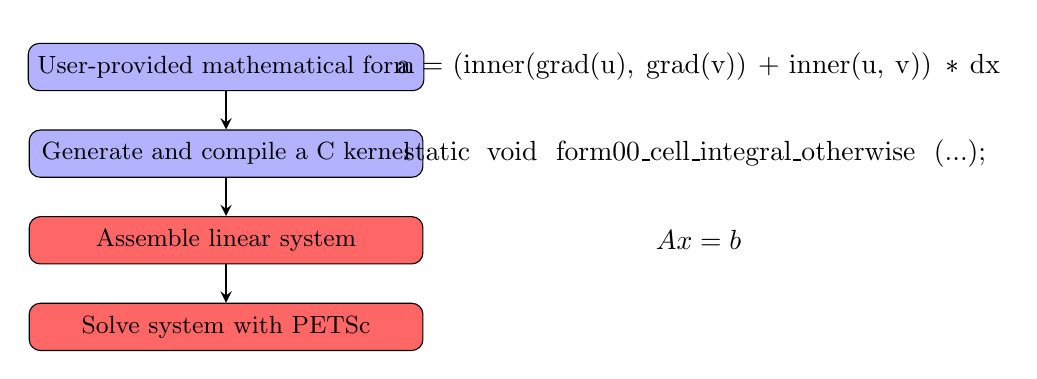
\begin{tikzpicture}
      \node (start) [node] {\small User-provided mathematical form};
      \node (codegen) [node, below of=start, yshift=-0.1cm] {\small Generate and compile a C kernel};
      \node (assemble) [expensivenode, below of=codegen, yshift=-0.1cm] {\small Assemble linear system};
      \node (solve) [expensivenode, below of=assemble, yshift=-0.1cm] {\small Solve system with PETSc};

      \draw [arrow] (start) -- (codegen);
      \draw [arrow] (codegen) -- (assemble);
      \draw [arrow] (assemble) -- (solve);

      \node (rstart) [empty, right of=start, xshift=5cm] {\lstinline{a = (inner(grad(u), grad(v)) + inner(u, v)) * dx}};
      \node (rcodegen) [empty, right of=codegen, xshift=5cm] {\lstinline{static void form00_cell_integral_otherwise(...);}};
      \node (rassemble) [empty, right of=assemble, xshift=5cm] {$Ax = b$};
    \end{tikzpicture}
  \end{center}

\end{frame}

\begin{frame}{Assumed performance characteristics}

  \begin{itemize}
    \item Latencies due to Python and code generation (amortized)
    \item Computations memory bound in the majority of cases
    \item MPI implementations for assembly and solve are good
  \end{itemize}

\end{frame}

\begin{frame}{Aims for the workshops}

  \begin{itemize}
    \item Study performance characteristics of the generated code and PETSc solvers
    \item Verify that MPI implementations are efficient (assembly and solve)
    \item Determine suitability of the tools for profiling Firedrake in the future
  \end{itemize}

\end{frame}

%%%%%%%%%%%%%%%%%%%%%%%%%%%%%%%%%%%%%%%%%%%%%%%%%%%%%%%%%%%%

\subsection{Problems}

\begin{frame}{Hurdles to using the profiling tools}
  \begin{itemize}
    \item Lots of things didn't work
    \item Many of the profiling tools assume C/C++/Fortran
  \end{itemize}
\end{frame}

\begin{frame}{What did/didn't work?}
  \centering
  \begin{tabular}{l|c|c}
    \textbf{Tool} & \textbf{Did it work?} & \textbf{Did it generate any insights?} \\
    \hline
    Intel VTune & No & No \\
    MAQAO & No & No \\
    MUST & Partially & No \\
    Scalasca & Skipped & No \\
    \hline
    Vampir & Yes & Some \\
    Allinea DDT & Yes & Some \\
    \hline
    Score-P & Yes & Yes \\
    Likwid & Yes & Yes
  \end{tabular}
\end{frame}

%%%%%%%%%%%%%%%%%%%%%%%%%%%%%%%%%%%%%%%%%%%%%%%%%%%%%%%%%%%%

\subsection{Insights}

\begin{frame}{Score-P}
  \begin{itemize}
    \item Told us we have great load balancing
    \item CUBE visualiser is very powerful
    \item It has Python bindings
  \end{itemize}
\end{frame}

\begin{frame}{Likwid}
  \begin{columns}[T]
    \begin{column}{0.5\textwidth}
      \vspace{-2em}

      \begin{figure}
	\centering
	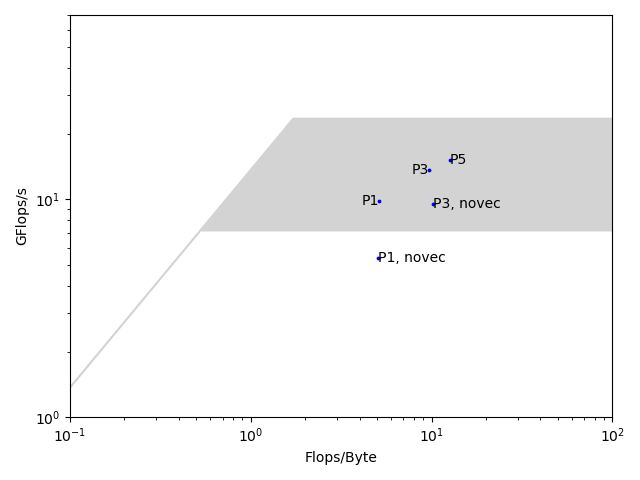
\includegraphics[width=0.8\textwidth]{roofline}
	\caption{Roofline plot for matrix-free assembly.}
      \end{figure}
    \end{column}
    %
    \begin{column}{0.35\textwidth}
      \begin{itemize}
	\item Easy to get working
	\item Very powerful
	\item Python bindings
      \end{itemize}
    \end{column}
  \end{columns}
\end{frame}

% --------------------------------------------------------------------------------

\subsection{Conclusions}

\begin{frame}{Takeaways}
  \textbf{The bad:}
  \begin{itemize}
    \item Sadly no performance gains made over the workshops
    \item Python/code generation causes lots of issues
    \item Did not investigate PETSc solvers as much as we would have liked
  \end{itemize}
  
  \vspace{1em}

  \textbf{The good:}
  \begin{itemize}
    \item Initial performance assumptions were largely verified
    \item We really liked Score-P and Likwid (Python bindings!) - we will try to use them more
    \item We learned a lot!
  \end{itemize}
\end{frame}

\begin{frame}{And lastly...}
  \begin{columns}[T]
    \begin{column}{0.45\textwidth}
      \begin{center}
	\vspace{3.5em}

	\textbf{A big thank you to the organisers and demonstrators!}

	\vspace{2em}

	Any questions?
      \end{center}
    \end{column}
    %
    \begin{column}[T]{0.45\textwidth}
      
\includegraphics[width=0.8\textwidth]{firedrake}
    \end{column}
  \end{columns}
\end{frame}

\subsection{Appendix}

\begin{frame}{Appendix: Allinea DDT}
  \vspace{-1em}
  \begin{columns}[T]
    \begin{column}[T]{0.45\textwidth}
      \begin{figure}
	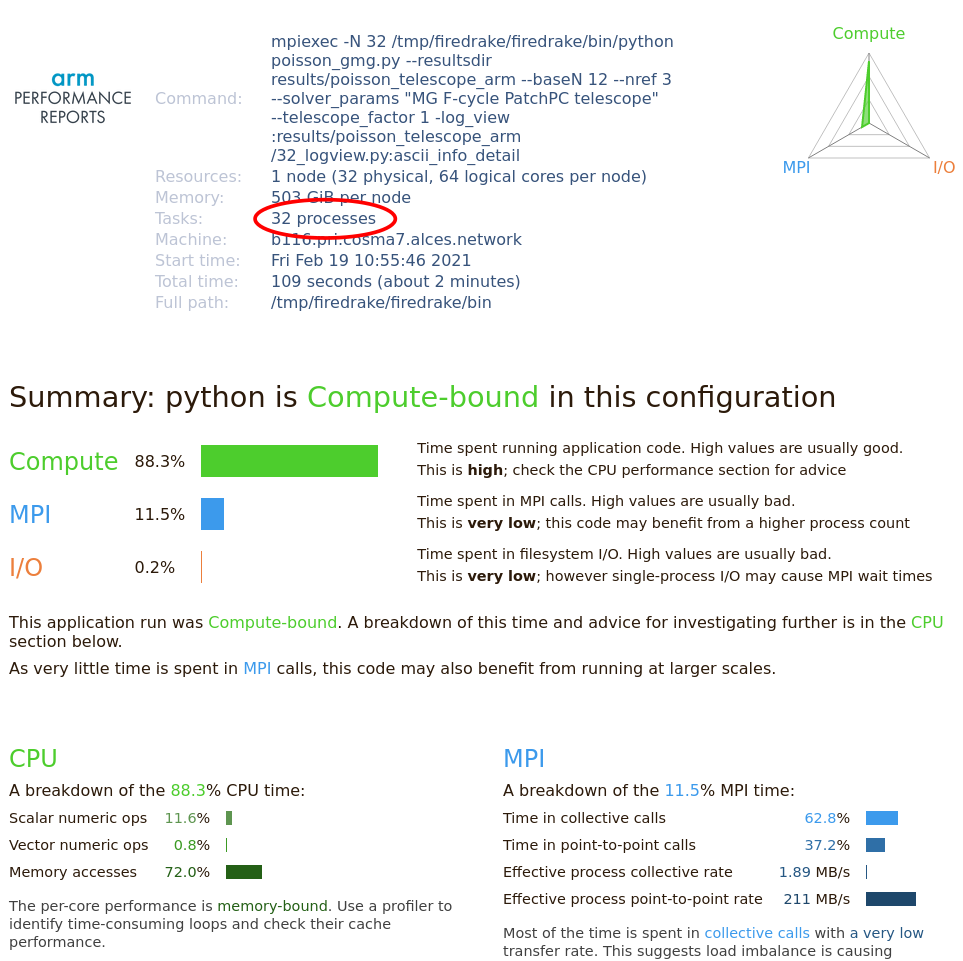
\includegraphics[width=\textwidth]{ddt_32_circled}
      \end{figure}
    \end{column}
    %
    \quad
    \begin{column}[T]{0.45\textwidth}
      \begin{figure}
	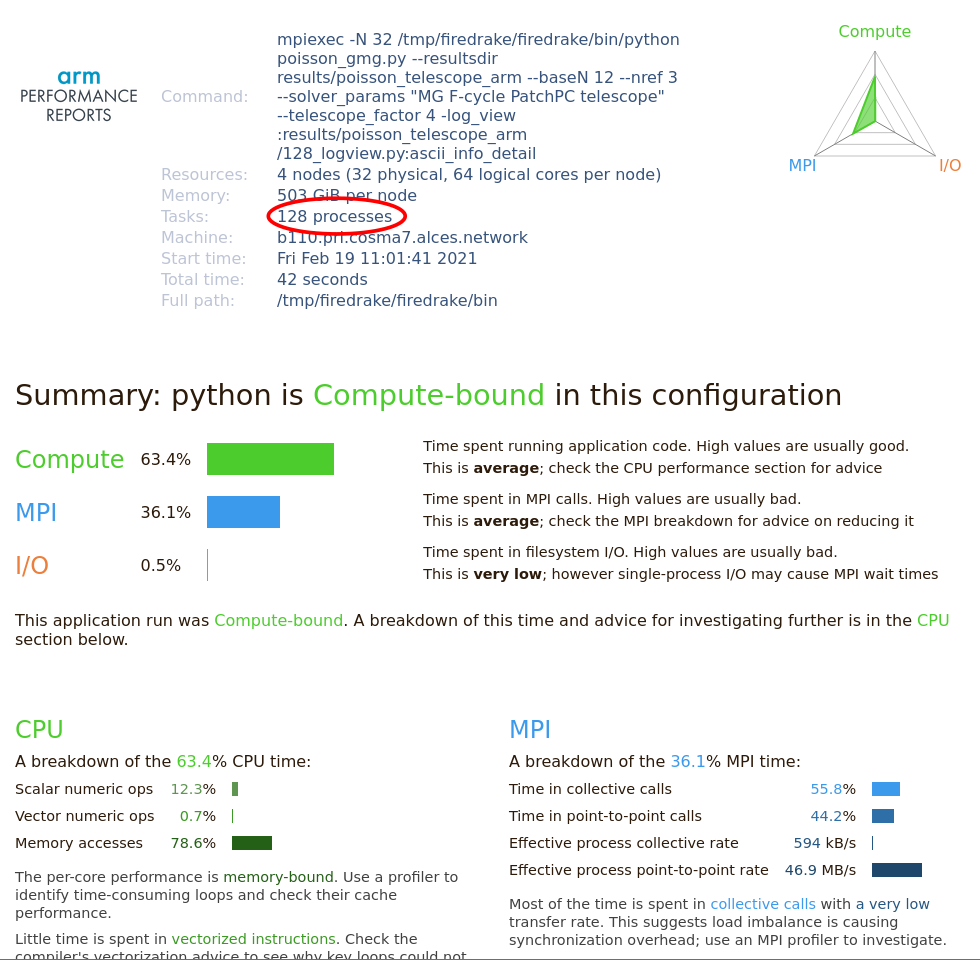
\includegraphics[width=\textwidth]{ddt_128_circled}
      \end{figure}
    \end{column}
  \end{columns}
\end{frame}

\end{document}
